\documentclass[11pt,letterpaper]{article}

\usepackage[margin=1in]{geometry}
\usepackage{enumitem}
\usepackage{hyperref}
\usepackage{amsmath}
\usepackage{amssymb}
\usepackage{booktabs}
\usepackage{float}
\usepackage{listings}
\usepackage{xcolor}
\usepackage{tikz}
\usetikzlibrary{calc, arrows.meta}

\title{16.07 Dynamics Problem Set 7}
\author{Due Friday, December 4}
\date{}

% vector / matrix shorthands (same as Problem Set 6)
\newcommand{\bw}{\boldsymbol{\omega}}
\newcommand{\Bw}{{}^{B}\boldsymbol{\omega}}
\newcommand{\bh}{\mathbf{h}}
\newcommand{\Nht}{{}^{N}\mathbf{h}}
\newcommand{\bJ}{\mathbf{J}}
\newcommand{\bA}{\mathbf{A}}
\newcommand{\ba}{\mathbf{a}}
\newcommand{\bq}{\mathbf{q}}
\newcommand{\bx}{\mathbf{x}}
\newcommand{\bu}{\mathbf{u}}
\newcommand{\bB}{\mathbf{B}}
\newcommand{\bM}{\mathbf{M}}
\newcommand{\br}{\mathbf{r}}
\newcommand{\bv}{\mathbf{v}}
\newcommand{\bF}{\mathbf{F}}
\newcommand{\Nr}{{}^{N}\mathbf{r}}
\newcommand{\Nrd}{{}^{N}\dot{\mathbf{r}}}
\newcommand{\Nrdd}{{}^{N}\ddot{\mathbf{r}}}
\newcommand{\vrel}{\mathbf{v}_{\text{rel}}}
\newcommand{\bomE}{\boldsymbol{\omega}_{\oplus}}

\begin{document}

\maketitle

\noindent In Problem Set 6, you built a six-degree-of-freedom simulation of a Dragon-like spacecraft orbiting a perfectly spherical Earth in a vacuum. In Question 1, we'll add the two most important perturbations in low-Earth orbit to your Dragon model: the Earth's equatorial bulge ($J_2$) and atmospheric drag. You'll see how much each one changes the orbit over a day. In Question 2, you'll derive the equations of motion for the circular restricted three-body problem (CR3BP), then use them to simulate the halo orbit flown by NASA's CAPSTONE spacecraft.

\section*{Question 1: Perturbations in Low-Earth Orbit}

We'll keep all the notation, vehicle parameters, and initial conditions from Problem Set 6. As before, the state is $\bx = [\Nr^T\;\,\ba^T\;\,\Nrd^T\;\,\Bw^T]^T \in \mathbb{R}^{13}$, the thrusters are off ($\bu = \mathbf{0}$), and the vehicle starts in the ISS-like circular orbit from Problem Set 6, Part 3. We'll take the $\hat n_3$ axis of the ECI frame $N$ to be along the Earth's spin axis, so the equator is the $\hat n_1$--$\hat n_2$ plane.

\paragraph{The $J_2$ perturbation.} The Earth is not a perfect sphere. Its rotation makes it bulge at the equator, with an equatorial radius about 21~km larger than its polar radius. To leading order, this adds a term to the gravitational potential that depends on latitude. The strength of this term is set by a dimensionless coefficient $J_2$. The resulting extra acceleration of the vehicle, in ECI components with $\Nr = [x\;\,y\;\,z]^T$ and $r = \lVert\Nr\rVert$, is
\begin{equation}
{}^{N}\ba_{J_2} = -\frac{3}{2}\,\frac{J_2\,\mu\,R_\oplus^2}{r^5}
\begin{bmatrix}
x\left(1 - 5\,\dfrac{z^2}{r^2}\right) \\[8pt]
y\left(1 - 5\,\dfrac{z^2}{r^2}\right) \\[8pt]
z\left(3 - 5\,\dfrac{z^2}{r^2}\right)
\end{bmatrix},
\label{eq:j2}
\end{equation}
where $R_\oplus$ is the Earth's equatorial radius. (We'll keep $\mathbf{a}$ for the attitude quaternion, so we'll write accelerations with a subscript, as in ${}^{N}\ba_{J_2}$.)

\paragraph{Atmospheric drag.} At 420~km, the atmosphere is very thin, but the vehicle moves through it at almost 8~km/s. The drag force is
\begin{equation}
{}^{N}\bF_D = -\frac12\,\rho\,C_D\,A\,\lVert\vrel\rVert\,\vrel,
\qquad
\vrel = \Nrd - \bomE\times\Nr,
\label{eq:drag}
\end{equation}
where $\rho$ is the local air density, $C_D$ is the drag coefficient, and $A$ is the vehicle's cross-sectional area. The atmosphere rotates with the Earth, so the drag depends on the velocity $\vrel$ of the vehicle \emph{relative to the air}, where ${}^{N}\bomE = [0\;\,0\;\,\omega_\oplus]^T$ is the Earth's angular velocity.

To keep things simple, we'll make two approximations:
\begin{itemize}
    \item \textbf{Spherical spacecraft.} We'll model the vehicle's aerodynamics as a sphere of radius $R_s = 2$~m (about Dragon's radius), centered at the center of mass $O$. A sphere presents the same cross-section $A = \pi R_s^2$ from every direction, so the drag force doesn't depend on the attitude. Since the drag acts through $O$, it also produces no torque.
    \item \textbf{Exponential atmosphere.} We'll fit an exponential density model around the starting altitude,
    \begin{equation}
    \rho(h) = \rho_0 \exp\!\left(-\frac{h - h_0}{H}\right), \qquad h = \lVert\Nr\rVert - R_\oplus,
    \label{eq:rho}
    \end{equation}
    where $H$ is the \emph{scale height}, the altitude change over which the density falls by a factor of $e$. The values in Table~\ref{tab:q1} are typical of moderate solar activity. The real density at this altitude can change by a factor of ten or more depending on ``space weather.''
\end{itemize}
The rotational dynamics are the same as in Problem Set 6.

\begin{table}[H]
\centering
\small
\begin{tabular}{lll}
\toprule
Quantity & Symbol & Value \\
\midrule
Earth's equatorial radius & $R_\oplus$ & $6{,}378{,}137$~m \\
Second zonal harmonic & $J_2$ & $1.08262668\times10^{-3}$ \\
Earth's rotation rate & $\omega_\oplus$ & $7.292115\times10^{-5}$~rad/s \\
Drag coefficient & $C_D$ & 2.2 \\
Sphere radius & $R_s$ & 2.0~m \\
Reference altitude & $h_0$ & 420~km \\
Density at $h_0$ & $\rho_0$ & $2.0\times10^{-12}$~kg/m$^3$ \\
Scale height & $H$ & 59~km \\
\bottomrule
\end{tabular}
\caption{Parameters for Question 1. All other values ($\mu$, $m$, $\bJ$, and the initial conditions) are the same as in Problem Set 6.}
\label{tab:q1}
\end{table}

\begin{enumerate}[label=(\alph*)]
    \item \textbf{Equations of motion:} Add $J_2$ and drag to Newton's 2nd law from Problem Set 6, Part 2(a). Then update the manipulator form from Problem Set 6, Part 2(b). The two perturbations go in different places:
    \begin{itemize}
        \item The $J_2$ acceleration goes in the gravity vector $\mathbf{g}(\bq)$. Like point-mass gravity, it's a conservative force that comes from a potential and depends only on the vehicle's position.
        \item The drag force goes on the right-hand side, as an external force. It's non-conservative: it removes energy from the orbit.
    \end{itemize}
    The manipulator form becomes
    \[
    \bM\,\dot\bv + \mathbf{c}(\bq,\bv) + \mathbf{g}(\bq) = \bB(\bq)\,\bu + \mathbf{f}_D(\bq,\bv),
    \]
    where $\mathbf{f}_D \in \mathbb{R}^6$ is the drag wrench. Write out the new $\mathbf{g}(\bq)$ and $\mathbf{f}_D(\bq,\bv)$.

    \item \textbf{Simulation:} Update your function $\mathbf{f}(\bx,\bu)$ so that each perturbation can be switched on and off. Using your explicit midpoint integrator from Problem Set 6 with $h = 0.1$~s, simulate 24 hours for four cases:
    \begin{enumerate}[label=(\roman*)]
        \item Two-body only (the model from Problem Set 6).
        \item $J_2$ only.
        \item Drag only.
        \item $J_2$ and drag.
    \end{enumerate}
    You don't need to store every step. Saving the state every 10~s (every 100 steps) is plenty for plotting. Each run should take at most a few minutes. Report the distance between the final position of each perturbed case and the final position of the two-body case. Which perturbation has a bigger effect on where the vehicle is after a day?

    \item \textbf{Altitude:} For all four cases, plot the altitude $h(t) = \lVert\Nr(t)\rVert - R_\oplus$ against time over the 24 hours.

    \item \textbf{RAAN:} The \emph{right ascension of the ascending node} (RAAN), $\Omega$, is the angle in the equatorial plane from $\hat n_1$ to the point where the orbit crosses the equator going north. It can be computed from the specific orbital angular momentum $\bh = \Nr\times\Nrd = [h_x\;\,h_y\;\,h_z]^T$:
    \[
    \Omega = \operatorname{atan2}\!\left(h_x,\,-h_y\right).
    \]
    For all four cases, plot $\Omega(t)$ against time over the 24 hours. (You may need to unwrap the angle.)
\end{enumerate}

\section*{Question 2: The Circular Restricted Three-Body Problem}

In the \emph{circular restricted three-body problem} (CR3BP), two massive bodies (the \emph{primaries}) with masses $m_1 > m_2$ orbit their common center of mass, the \emph{barycenter}, in circular orbits. A third body, such as a spacecraft, moves in their combined gravity field. Its mass is so small that it doesn't affect the motion of the primaries. The Earth--Moon system with a spacecraft is a good example. NASA's recent CAPSTONE mission and proposed Gateway lunar space station use orbits that are designed with this model.

\begin{figure}[h]
\centering
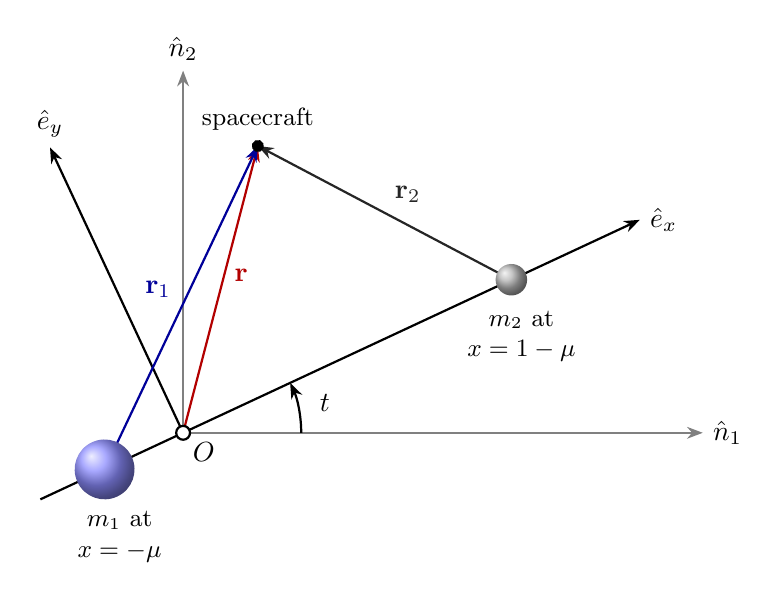
\begin{tikzpicture}[scale=1.0, >={Stealth[length=2mm]}]
    \def\th{25}
    % Inertial axes
    \draw[->, thick, gray] (0,0) -- (6.6,0) node[right, black] {$\hat n_1$};
    \draw[->, thick, gray] (0,0) -- (0,4.6) node[above, black] {$\hat n_2$};
    % Rotation angle
    \draw[->, thick] (1.5,0) arc[start angle=0, end angle=\th, radius=1.5];
    \node at (1.8,0.38) {$t$};
    % Rotating frame
    \begin{scope}[rotate=\th]
        \draw[->, thick] (-2.0,0) -- (6.4,0) node[right] {$\hat e_x$};
        \draw[->, thick] (0,0) -- (0,4.0) node[above] {$\hat e_y$};
        \coordinate (E) at (-1.1,0);
        \coordinate (M) at (4.6,0);
        \coordinate (S) at (2.4,2.9);
        % Position vectors
        \draw[->, thick, red!70!black] (0,0) -- (S) node[pos=0.55, right] {$\br$};
        \draw[->, thick, blue!60!black] (E) -- (S) node[pos=0.5, above left] {$\br_1$};
        \draw[->, thick, gray!30!black] (M) -- (S) node[pos=0.5, above right] {$\br_2$};
        % Primaries (sizes and positions not to scale)
        \shade[ball color=blue!45] (E) circle (0.38);
        \shade[ball color=gray!60] (M) circle (0.2);
        \filldraw[fill=black] (S) circle (2pt);
        \node[anchor=north, align=center, font=\small] at ($(E)+(0,-0.45)$) {$m_1$ at\\ $x=-\mu$};
        \node[anchor=north, align=center, font=\small] at ($(M)+(0,-0.3)$) {$m_2$ at\\ $x=1-\mu$};
        \node[above=2pt, font=\small] at (S) {spacecraft};
    \end{scope}
    % Barycenter
    \filldraw[fill=white, thick] (0,0) circle (2.5pt);
    \node[below right] at (0,0) {$O$};
\end{tikzpicture}
\caption{The CR3BP in nondimensional units. The rotating frame $R$ has its origin at the barycenter $O$ and turns with the primaries at unit angular velocity about $\hat e_z = \hat n_3$ (out of the page), so after time $t$ it has rotated by the angle $t$ relative to the inertial frame $N$. In $R$, the primaries sit at fixed points on the $\hat e_x$ axis. Drawing not to scale.}
\label{fig:cr3bp}
\end{figure}

\paragraph{The rotating frame.} The primaries move in circles in an inertial frame, but they stand still in a frame that rotates with them. Let $R$ be the frame with origin at the barycenter $O$, $\hat e_x$ pointing from $m_1$ to $m_2$, and $\hat e_z$ along the primaries' orbital angular momentum (Fig.~\ref{fig:cr3bp}). This frame rotates at the primaries' constant orbital rate $n$ about $\hat e_z$. We'll describe the spacecraft by its position $\br = x\,\hat e_x + y\,\hat e_y + z\,\hat e_z$ in $R$.

\paragraph{Nondimensional units.} The CR3BP has a single parameter, the \emph{mass ratio}
\[
\mu = \frac{m_2}{m_1 + m_2}.
\]
(Careful: this is not the same $\mu$ as the Earth's gravitational parameter in Question 1.) We'll choose units in which everything else is 1:
\begin{itemize}
    \item The unit of mass is $m_1 + m_2$.
    \item The unit of length $L^*$ is the distance between the primaries.
    \item The unit of time $T^*$ is set by the primaries' orbital period $P$: $T^* = P/2\pi$. The primaries complete one orbit every $2\pi$ time units, so their orbital rate is $n = 1$. With these units, the gravitational constant (``big G'') is $G = 1$.
\end{itemize}
For the Earth--Moon system, use
\[
\mu = 0.012150585609624, \qquad L^* = 384{,}400~\text{km}, \qquad T^* = 375{,}190~\text{s} \approx 4.343~\text{days}.
\]
In these units, the primaries sit at fixed points on the $\hat e_x$ axis, $m_1$ at $x = -\mu$ and $m_2$ at $x = 1-\mu$, so the spacecraft's distances from them are
\[
r_1 = \sqrt{(x+\mu)^2 + y^2 + z^2}, \qquad r_2 = \sqrt{(x-1+\mu)^2 + y^2 + z^2}.
\]

\begin{enumerate}[label=(\alph*)]
    \item \textbf{Inertial velocity:} The kinetic energy in the Lagrangian must be computed from the spacecraft's velocity relative to the \emph{inertial} frame. Using the transport theorem with ${}^{N}\bw^{R} = \hat e_z$, write the spacecraft's inertial velocity ${}^{N}\dot\br$ in $R$-frame components, in terms of $x$, $y$, $z$, $\dot x$, $\dot y$, and $\dot z$.

    \item \textbf{The Lagrangian:} Write the spacecraft's kinetic energy $T$ and gravitational potential energy $V$, per unit mass, and the Lagrangian $\mathcal{L} = T - V$, in terms of the rotating-frame coordinates $(x, y, z)$ and their rates.

    \item \textbf{The effective potential:} Expand $\mathcal{L}$ and group its terms by their order in the velocities $(\dot x, \dot y, \dot z)$:
    \[
    \mathcal{L} = \mathcal{L}_2 + \mathcal{L}_1 + \mathcal{L}_0,
    \]
    where $\mathcal{L}_2$ is quadratic in the velocities, $\mathcal{L}_1$ is linear in them, and $\mathcal{L}_0$ doesn't depend on them at all. Show that $\mathcal{L}_0$ can be written as $\mathcal{L}_0 = U(x,y,z)$, where
    \[
    U(x, y, z) = \frac12\left(x^2 + y^2\right) + \frac{1-\mu}{r_1} + \frac{\mu}{r_2}
    \]
    is called the \emph{effective potential}. (Note the sign convention: $-U$ plays the role of a potential energy.) Where does the $\frac12(x^2 + y^2)$ term come from physically?

    \item \textbf{Equations of motion:} Apply the Euler--Lagrange equation
    \[
    \frac{d}{dt}\left(\frac{\partial\mathcal{L}}{\partial\dot q_j}\right) - \frac{\partial\mathcal{L}}{\partial q_j} = 0
    \]
    to each of $q_j = x, y, z$, and show that the equations of motion are
    \[
    \ddot x - 2\dot y = \frac{\partial U}{\partial x}, \qquad
    \ddot y + 2\dot x = \frac{\partial U}{\partial y}, \qquad
    \ddot z = \frac{\partial U}{\partial z}.
    \]
    Then write out the three partial derivatives of $U$ explicitly.

    \item \textbf{CAPSTONE's halo orbit:} Near each of the collinear Lagrange points there's a family of periodic, three-dimensional \emph{halo orbits}. The members of the $L_2$ family that pass closest to the Moon are called \emph{near-rectilinear halo orbits} (NRHOs). In November 2022, NASA's CAPSTONE CubeSat became the first spacecraft to fly in one. It's the same orbit planned for Gateway: a southern $L_2$ NRHO that completes 9 orbits for every 2 lunar synodic months, passing about 3{,}200~km from the Moon's center over the north pole and about 70{,}000~km over the south pole. In the CR3BP, this orbit starts at apolune with
    \[
    \begin{gathered}
    x_0 = 1.022028213459, \qquad y_0 = 0, \qquad z_0 = -0.182101401321, \\
    \dot x_0 = 0, \qquad \dot y_0 = -0.103270951324, \qquad \dot z_0 = 0,
    \end{gathered}
    \]
    and has period $T = 1.511199434655$ (about 6.56 days).
    
Write the equations of motion as a first-order ODE in the state $[x\;\,y\;\,z\;\,\dot x\;\,\dot y\;\,\dot z]^T$, and integrate them for one period using \texttt{ode45} or \texttt{ode113} in MATLAB, or \texttt{solve\_ivp} with \texttt{method='DOP853'} in Python. Use tight tolerances: \texttt{RelTol} and \texttt{AbsTol} (\texttt{rtol} and \texttt{atol}) of $10^{-12}$. Plot the orbit in 3D in the rotating frame, along with the Moon's position, and convert the axes to kilometers. Verify that the spacecraft returns to its initial state after one period. What are its closest and farthest distances from the Moon's center?

\end{enumerate}

\end{document}
